\section{A controlled context-to-action experiment}
\begin{figure}[t]
\centering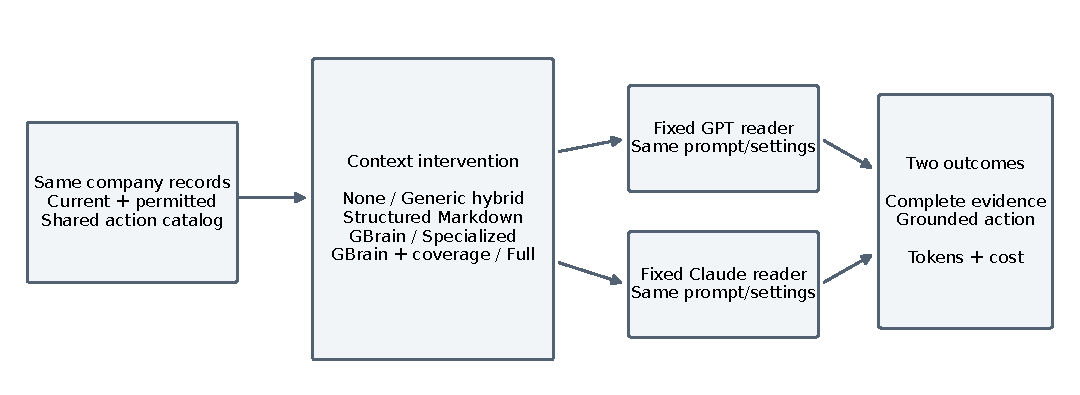
\includegraphics[width=\linewidth]{figures/integrated/design.pdf}
\caption{Shared sources and task, changed evidence packet, fixed reader. Context completeness is measured before the reader; action groundedness is measured afterward. The pipeline does not imply commercial causality.}
\label{fig:design}
\end{figure}
\subsection{Data, boundaries and task}
We instantiate 33 fresh fictional company worlds, 264 queries, across renewal, partner and compliance families. Four development worlds use hiring and migration. The new main worlds are disjoint from both the pilot and earlier experiments; the relation families were used in historical development and are not previously unseen research concepts. Each world contains a seller, a target account, a shared four-action catalog and 12--36 distractor records. Four conditions are answerable and four require withholding. Conditions span initial context, weak feedback, policy revision, account requalification, evidence correction, restricted evidence, objective change and policy conflict.

Every method receives the same verified events with source ID, valid time, observed time, authority and access scope. A shared visibility/supersession function removes future, superseded and unauthorized records before selection. Consequently, the experiment measures \emph{selection after common maintenance}; it does not establish that one memory discovers updates or permissions better. Weak feedback cannot become approved policy. Conflicting current values remain explicit. The data are original, AI-assisted templates with deterministic construction labels cross-checked by Python and SQLite implementations, not customer observations or human annotations.

A reader returns at most one action, source bindings, missing information and a short explanation. An action must match the objective and resource allowance and satisfy its own prerequisites and cross-field equalities. Multiple catalog actions may be acceptable. The public catalog supplies requirements to every arm; hidden labels and future events never enter requests. Schema validity, evidence grounding and prerequisite satisfaction are machine-checkable. A separate post-hoc mock executor checks internal workflow consistency, not outreach effectiveness; the scorer’s catalog-feasibility receipt alone is not execution.

\subsection{Seven contexts, two fixed readers}
\begin{table}[t]
\centering\small
\begin{tabularx}{\linewidth}{@{}p{.21\linewidth}X@{}}
\toprule
Treatment & Executed mechanism \\
\midrule
No company context & Shared task/catalog only; information-availability reference \\
Generic hybrid & BM25 plus real dense embeddings; reciprocal-rank fusion ($k=60$) \\
Structured Markdown & Lossless entity files; generic ranking diversified by relation/authority \\
GBrain search & Actual pinned PGLite balanced hybrid search, same real vectors \\
Specialized coverage & Generic ranking prioritized by public action prerequisites, then diversified \\
GBrain + coverage & The identical prerequisite-coverage layer over native GBrain candidates \\
Full current context & Every permitted seller/account record; larger-resource reference \\
\bottomrule
\end{tabularx}
\caption{Only context selection changes within a reader. All arms share a strong domain-aware prompt; Generic is therefore also the prompt-specialized control.}
\label{tab:arms}
\end{table}

BM25 and reciprocal-rank fusion follow standard retrieval practice~\citep{robertson2009,cormack2009}. All dense retrieval uses actual \texttt{text-embedding-3-small} vectors with 1,024 dimensions. GBrain\footnote{\url{https://github.com/garrytan/gbrain}; MIT-licensed upstream, installed separately.} is pinned to \texttt{531b3b1} (version 0.60.380.0); its semantic path is verified in saved receipts. We exercise native search over common atomic records, with reranking off and no extracted source graph, synthesis or native ingestion. This is a component evaluation, not GBrain's best complete configuration.

The specialized layer prioritizes relation/authority groups required by feasible catalog actions. It never filters by the correct value or reads a label. Generic file diversity covers relation/authority groups without catalog priorities, making it an essential falsifier: generic coverage may suffice. The controlled Markdown representation is lossless and deterministic, not an LLM-generated wiki or a claimed Karpathy implementation. Section~\ref{sec:external} separately evaluates actual wiki compilation.

Primary evidence allowance is 2,048 UTF-8 bytes in the same canonical record encoding. Instructions and catalog are common and excluded from that allowance. Whole records are packed without truncating their contents. This is an equal serialization budget, \emph{not} exact tokenizer equality; actual provider tokens and costs are reported. Retrieval-only sweeps use 1,024, 2,048, 4,096 and 8,192 bytes. Full context and no context are explicitly unequal-information references.

The readers are \texttt{gpt-6.1-sol} (low reasoning) and \texttt{claude-sonnet-5-5} (provider defaults), each with 2,048 maximum output tokens and the same public JSON schema. Within each provider, settings and prompts are identical across arms. There is one request per case/arm/provider, shuffled deterministically; no answer retries or external tools. A Claude/GPT difference would also include different provider defaults and tokenizers, so our primary contrasts are \emph{within} each model.

\subsection{Outcomes, precision and accounting}
Context quality is the proportion of answerable queries whose packet contains at least one complete current support set. Grounded decision correctness counts a supported eligible recommendation on answerable cases and correct withholding on negative cases. We separately report positive coverage, inappropriate abstention, unsupported recommendations, false apparent eligibility, failures and a deterministic validator's effect. The validator cannot import missing facts or repair citations. Scores are recomputed from raw saved responses without an LLM judge.

The completed pilot issued 448 requests. Its paired world-level SD selected 33 main worlds through the prespecified rule $n=\lceil(1.96s/0.075)^2\rceil$, rounded to a multiple of three and bounded 24--60. The main seed, code, input hashes and analysis were frozen before main requests. No resizing or outcome-based stopping follows. Paired differences use world means; 95\% bootstrap intervals resample worlds within family (10,000 draws). Exact paired sign tests for Specialized--Generic are Holm-adjusted across the two readers. Other contrasts are descriptive. Clustering does not turn templated worlds into real-company samples; degenerate intervals at a ceiling reflect the observed fixtures.

Costs use actual reported input, output and cache usage and official prices checked 22 October 2026. Both readers list \$2/M uncached input and \$10/M output; cache reads/writes are costed separately. Estimates are not reconciled invoices. Ingestion, queries and compilation are separated. All attempts, including the stopped serialization pilot and transport failures, remain available. Researcher-selected execution guards bound requests; they are not user-specified spending limits.
